\section*{Scope of this English edition}
This draft establishes one logical route in English for the core argument.
The complete English technical appendix is still in preparation and is not
included in this release. Accordingly, this document is not a self-contained
full proof: propositions that cite R-modules still require those detailed
derivations. The historical source is pinned
to commit \texttt{99408ee}. This is an editorial reconstruction of a candidate
proof, not a new assertion of independent mathematical validation.
Stable module identifiers locate the detailed source and arithmetic evidence.
The technical translation requires mathematical editing; preserving formulae
does not establish that a translation preserves every hypothesis or implication.

Appendix~\ref{app:M1} gives the only active normalization protocol.
The stronger one-shot global-clamping scheme is excluded from this reading
route. Global notation is fixed before the geometry begins. Auxiliary
parameters of a technical lemma are locally scoped: the same letter in two
lemmas never licenses transferring a hypothesis.

\begin{figure}[htbp]\centering
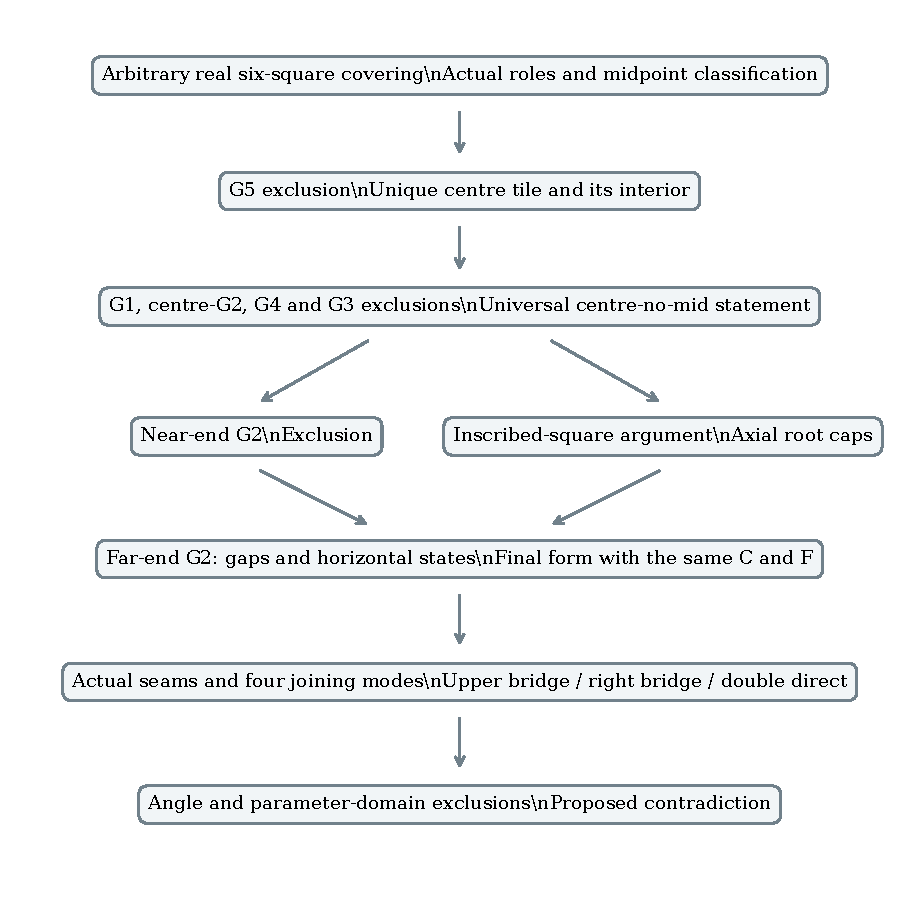
\includegraphics[width=.83\textwidth,height=.76\textheight,keepaspectratio]{figures/06_dependency_order.pdf}
\caption{The proposed logical dependency order. An arrow is a geometric
implication to check, not an arithmetic verification result.}
\label{fig:route}\end{figure}
